\subsection{23 августа.  Пер. Джалпаккол Северный (1А)}
\textit{Метеоусловия: утром ясно, тепло; после 16:00 туман, дождь; ночью ясно.}

\begin{figure}[h!]
	\centering
	\includegraphics[angle=0, width=0.7\linewidth]{../pics/mini_maps/23}
	\label{fig:mini_23}
\end{figure}


Подъём в 04:30, выход в 07:30. С места ночёвки на следующую ступень долины идёт довольно крутой подъём по помеченной турами тропе (рис.~\ref{fig:23augstart}); затем тропа выходит на моренные валы. Спустя 2 перехода участница Наташа Миронова сообщила руководителю о том, что у неё начались проблемы с коленями и высказала опасения, что пройти поход до конца она не сможет. \alert{(Уточнить у Кати время и симптомы.)} В 08:50 мы оказались на развилке троп (левая пхд тропа вела на каскадные озёра). Встретили семейную пару туристов с собакой, которые спускались с перевала через эти озёра. Там же сделали привал, на котором Наташе сделали противоотёчное тейпирование и выдали компрессионный наколенник.

\begin{figure}[h!]
	\centering
	\includegraphics[angle=0, width=0.7\linewidth]{../pics/23augstart}
	\caption{Путь подъёма к перевалу Джалпаккол Северный от места ночёвки. Фото из отчёта Королёва А.Э. \cite{Korolyov2018}}
	\label{fig:23augstart}
\end{figure}

Далее двигались по гребню моренного вала по слабомаркированной турами тропе. Путь был утомительным, но физически и технически несложным. В 13:16 (за 8 ходок от старта) подошли под перевальный взлёт, пересёкши два небольших плоских снежничка. Надели кошки. На самом перевале снега практически не было, ледник  оказался полностью открыт (рис.~\ref{fig:dzh_1}). Справа от ледника пхд шёл гребень моренного вала. Стандартный путь на этот перевал проходит именно по этому гребню, и --- далее характерным крюком в обход ледовой линзы, по снегу, вдоль разрушенного скального гребня с южной стороны перевала. Однако в нашем случае, когда снега на перевале не было, такой маршрут проходил бы по осыпи, что только затруднило бы движение. Что касается полоски снега под правой пхд стороной взлёта, то с левой своей стороны она граничила со льдом, а в верхней части упиралась в осыпь под разрушенными скалами, и на снегу виднелись <<струйки>> от скатившихся камней, самые крупные из которых были размером примерно с собак. Руководитель принял решение максимально избегать встречи с камнями, и скомандовал группе уходить косым траверсом на лёд. Под самой седловиной перевала в тот момент был небольшой снежный <<карман>>: спрессованный снег, частично вытаявший под большой гладкой скалой и сформировавший углубление с бортиком в форме полумесяца. После пересечения ледника участники заходили за бортик кармана, в понижение, и там в относительной безопасности снимали кошки (рис.~\ref{fig:DSC_0021}).

\begin{figure}[h!]
	\centering
	\includegraphics[width=0.7\linewidth]{../pics/dzh_1}
	\caption{Перевальный взлёт пер. Джалпаккол Северный}
	\label{fig:dzh_1}
\end{figure}

\begin{figure}[h!]	
	\centering
	\includegraphics[angle=0, width=0.7\linewidth]{../pics/gopro_dzh}
	\caption{Подъём по леднику}
	\label{fig:gopro_dzh}
\end{figure}

\begin{figure}[h!]	
	\centering
	\includegraphics[angle=0, width=0.7\linewidth]{../pics/DSC_0021}
	\caption{Группа в снежном кармане перед скальным участком перевала}
	\label{fig:DSC_0021}
\end{figure}

Подъём по леднику занял 20 минут (рис.~\ref{fig:gopro_dzh}), Последний участник зашёл за бортик снежного балкона в 14:48. Кошки сняли. Оставался финальный участок перевала: 10 метров лазания по сильно разрушенным скалам (рис.~\ref{fig:DSC_0021}).

Руководитель вышла на разведку без рюкзака, после чего группа командами по 2-3 человека поднялась на седловину. Поэтапный выпуск участников был связан с тем, что подъём на седловину проходил косым травером над тем самым балконом, прикрытым скалой, где расположилась группа, поэтому следовало быть предельно аккуратным. Руководитель и заместитель контролировали прохождение участниками подъёма на двух самых опасных участках и выпускали каждого следующего участника строго по команде. В 15:30 вся группа собралась на перевале (рис.~\ref{fig:DSC_0063}, \ref{fig:DSC_0069}).

\begin{figure}[h!]	
	\centering
	\includegraphics[angle=0, width=0.7\linewidth]{../pics/DSC_0063}
	\caption{Группа на пер. Джалпаккол Северный (1А$^\star$)}
	\label{fig:DSC_0063}
\end{figure}

\begin{figure}[h!]	
	\centering
	\includegraphics[angle=0, width=0.7\linewidth]{../pics/DSC_0069}
	\caption{Группа на пер. Джалпаккол Северный (1А$^\star$), вид в д.р. Кичкинекол Джалпаккольский}
	\label{fig:DSC_0069}
\end{figure}

\begin{figure}[h!]	
	\centering
	\includegraphics[angle=0, width=0.7\linewidth]{../pics/DSC_0041}
	\caption{Вид с перевала на спуск в д.р. Мырды}
	\label{fig:DSC_0041}
\end{figure}

В 16:15 начали спуск (рис.~\ref{fig:DSC_0041}). Перевальный взлёт Джалпаккола Северного со стороны р. Мырды представляет собой среднюю и мелкую осыпь. К озеру под перевалом спустились в 17:00 и стали обходить его справа пхд (по южному берегу). Увидели, как на берег озера вышла пара горных козлов. Тем временем начал опускаться туман, стал накрапывать мелкий дождь --- видимость сильно упала. Поскольку мы находились на ступени, дальнейший путь в целом не просматривался, поэтому, обходя озеро, ориентировались в том числе на точку выхода горных козлов, что оказалось хорошим решением. (рис.~\ref{fig:IMG_20240823_170306}). Бараньи лбы на восточной оконечности озера и далее по спуску проходили максимально аккуратно, так как от дождя камни стали скользкими. 
 
\begin{figure}[h!]	
	\centering
	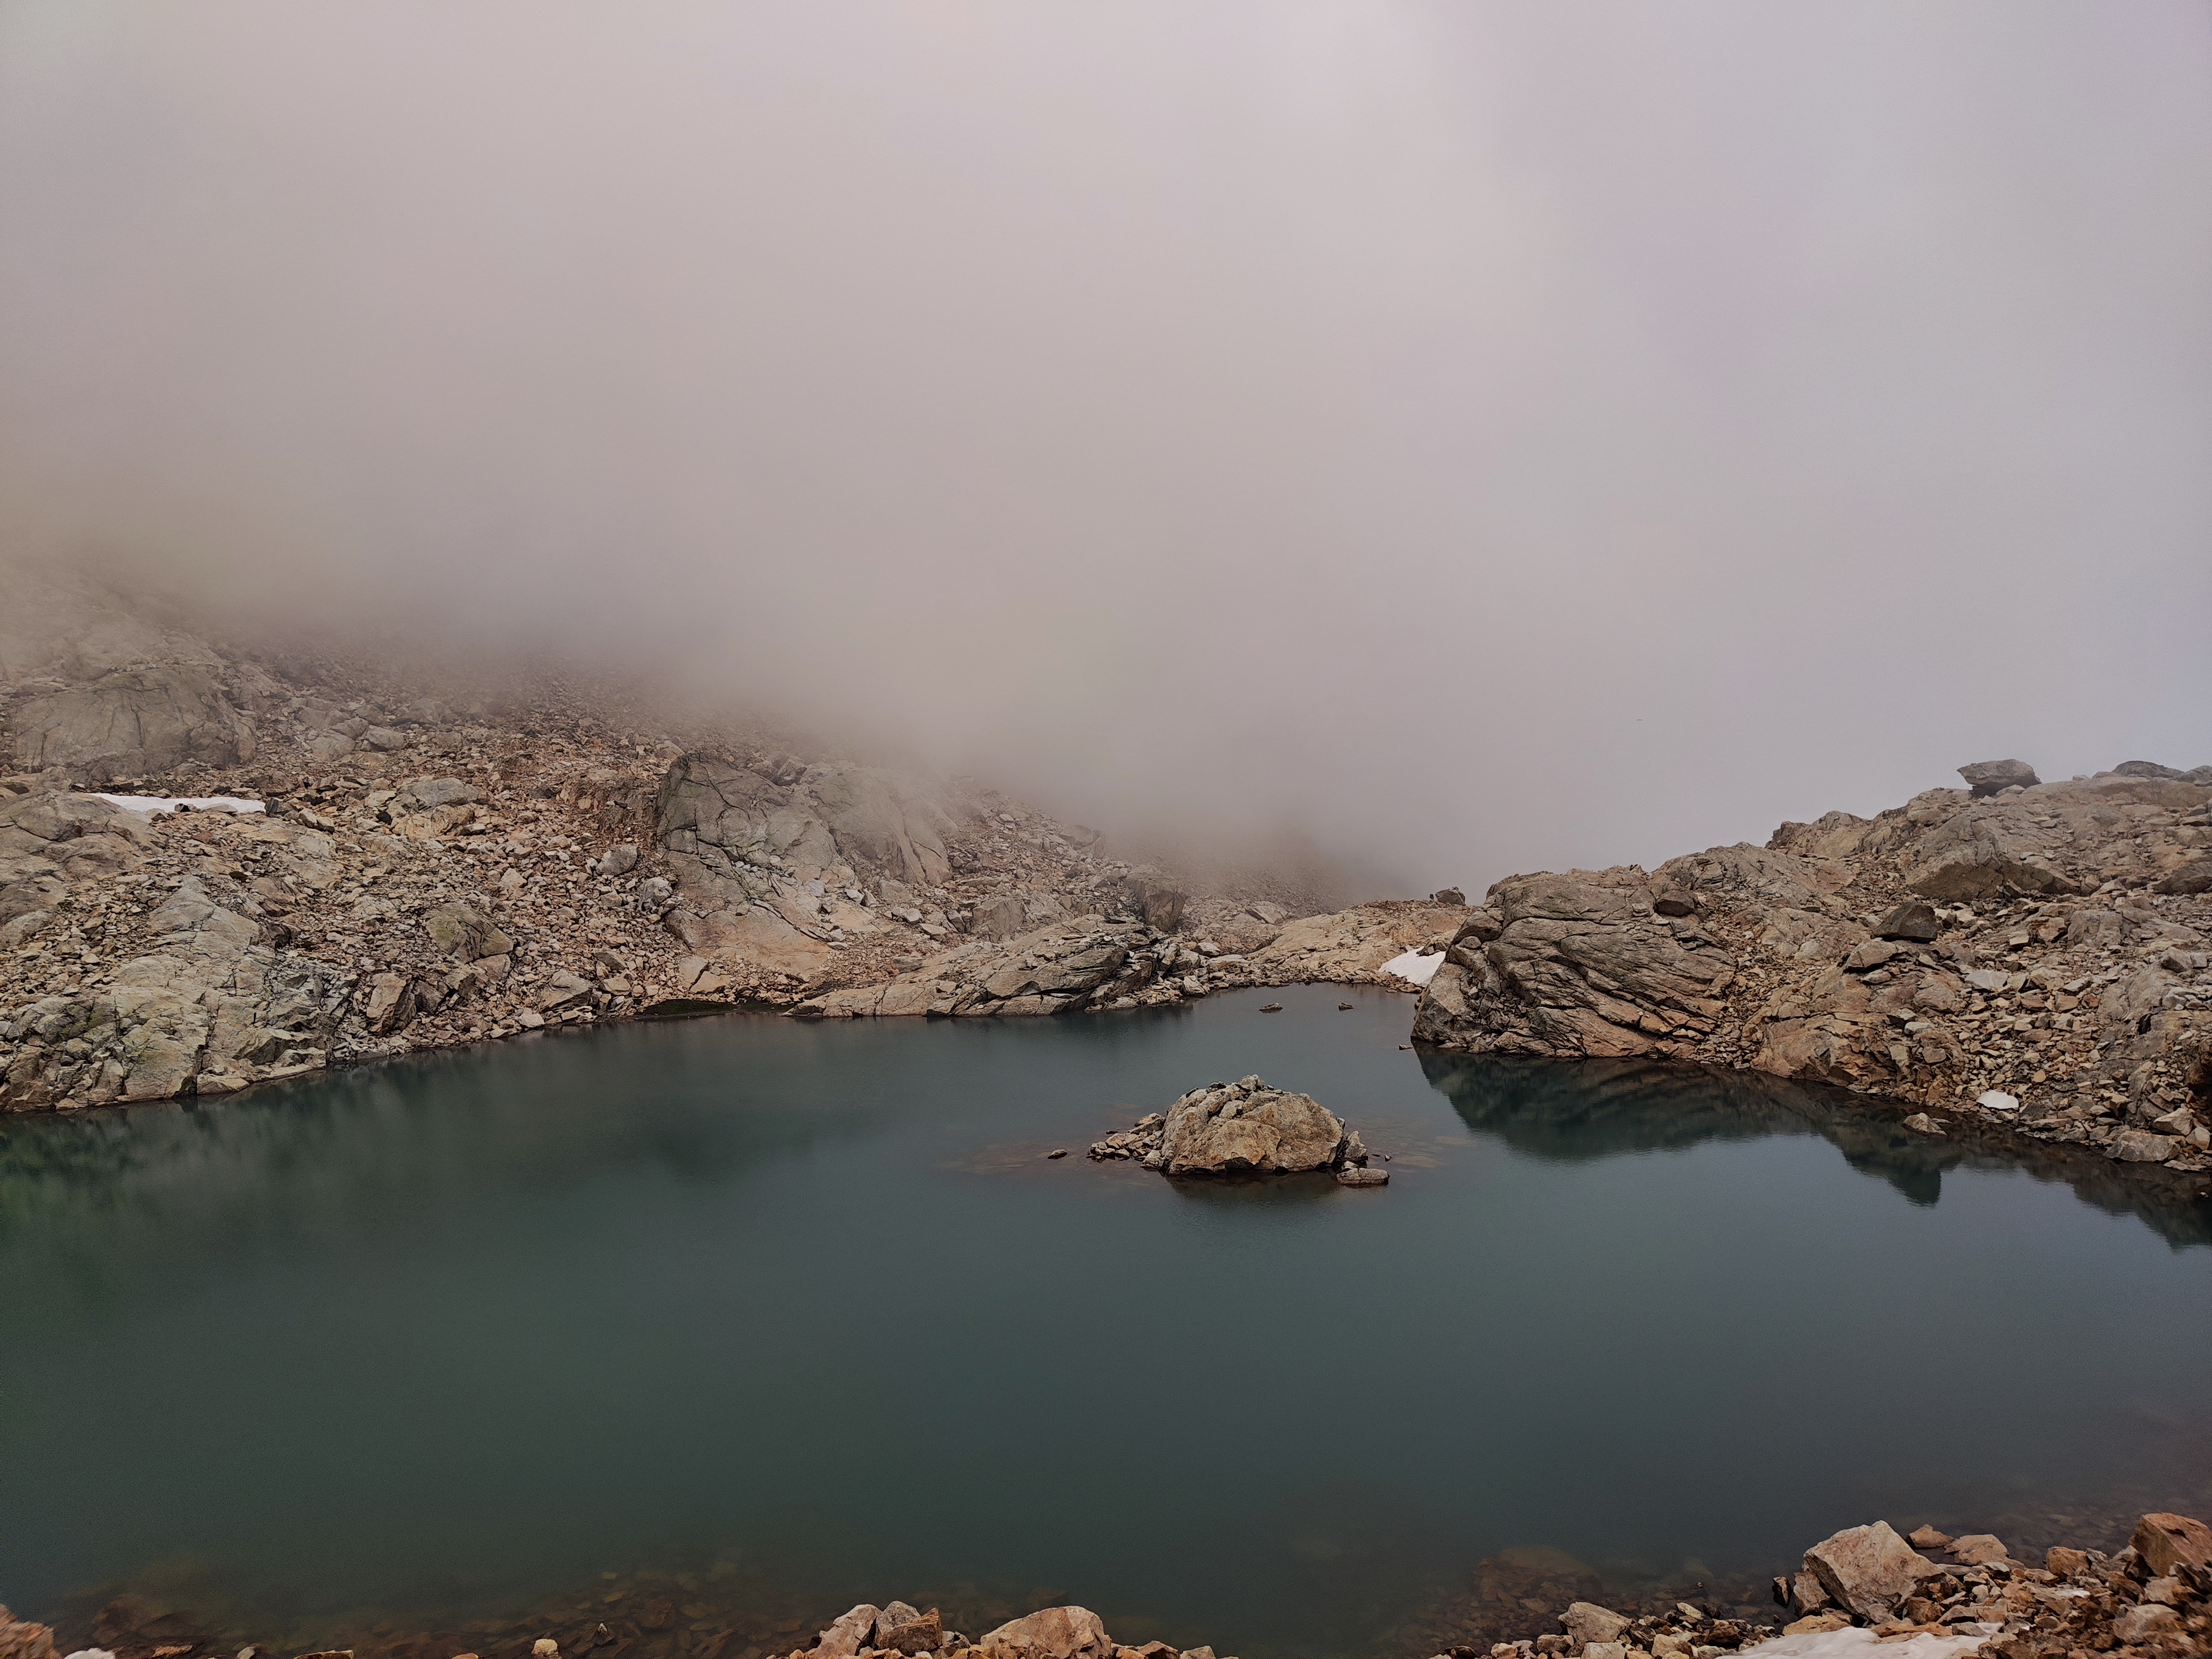
\includegraphics[angle=0, width=0.7\linewidth]{../pics/IMG_20240823_170306}
	\caption{Туман на озере под пер. Джалпаккол Северный}
	\label{fig:IMG_20240823_170306}
\end{figure} 

Дальнейший спуск отнял очень много сил, т.~к. из-за тумана шли практически полностью <<по приборам>> --- т.е. по навигатору --- с локальным ориентированием на местности в пределах 10--20~м. Спуск продолжал идти полностью по осыпи среднего и крупного размера; при этом на тропу либо так и не удалось выйти, либо она была крайне слабо читаемой. Добавляло сложности и то, что у Наташи болели колени, проблемы с которыми в условиях спуска по мокрым камням усугубились. 

С осыпи сошли в 18:10 , за 3 ходки с седловины перевала, довольно точно выйдя на тропу в зоне альпийского луга. Эта тропа идёт серпантином по склону, два раза обходя участки бараньих лбов. В условиях тумана и моросящего дождя спуск был довольно изматывающим физически и сильно изматывающим психологически. В зоне вторых бараньих лбов есть риск спустить камень на идущих ниже, поскольку тропа на этом участке идёт вниз практически не петляя. Этот этап занял 20 мин ЧХВ.

В 18:30 дошли до оборудованных стоянок на выполаживании травянисто-осыпного склона. (рис.~\ref{fig:IMG_20240823_184041}). Координаты м.н.: N~43.274531\degree, E~42.122488\degree.

\begin{figure}[h!]	
	\centering
	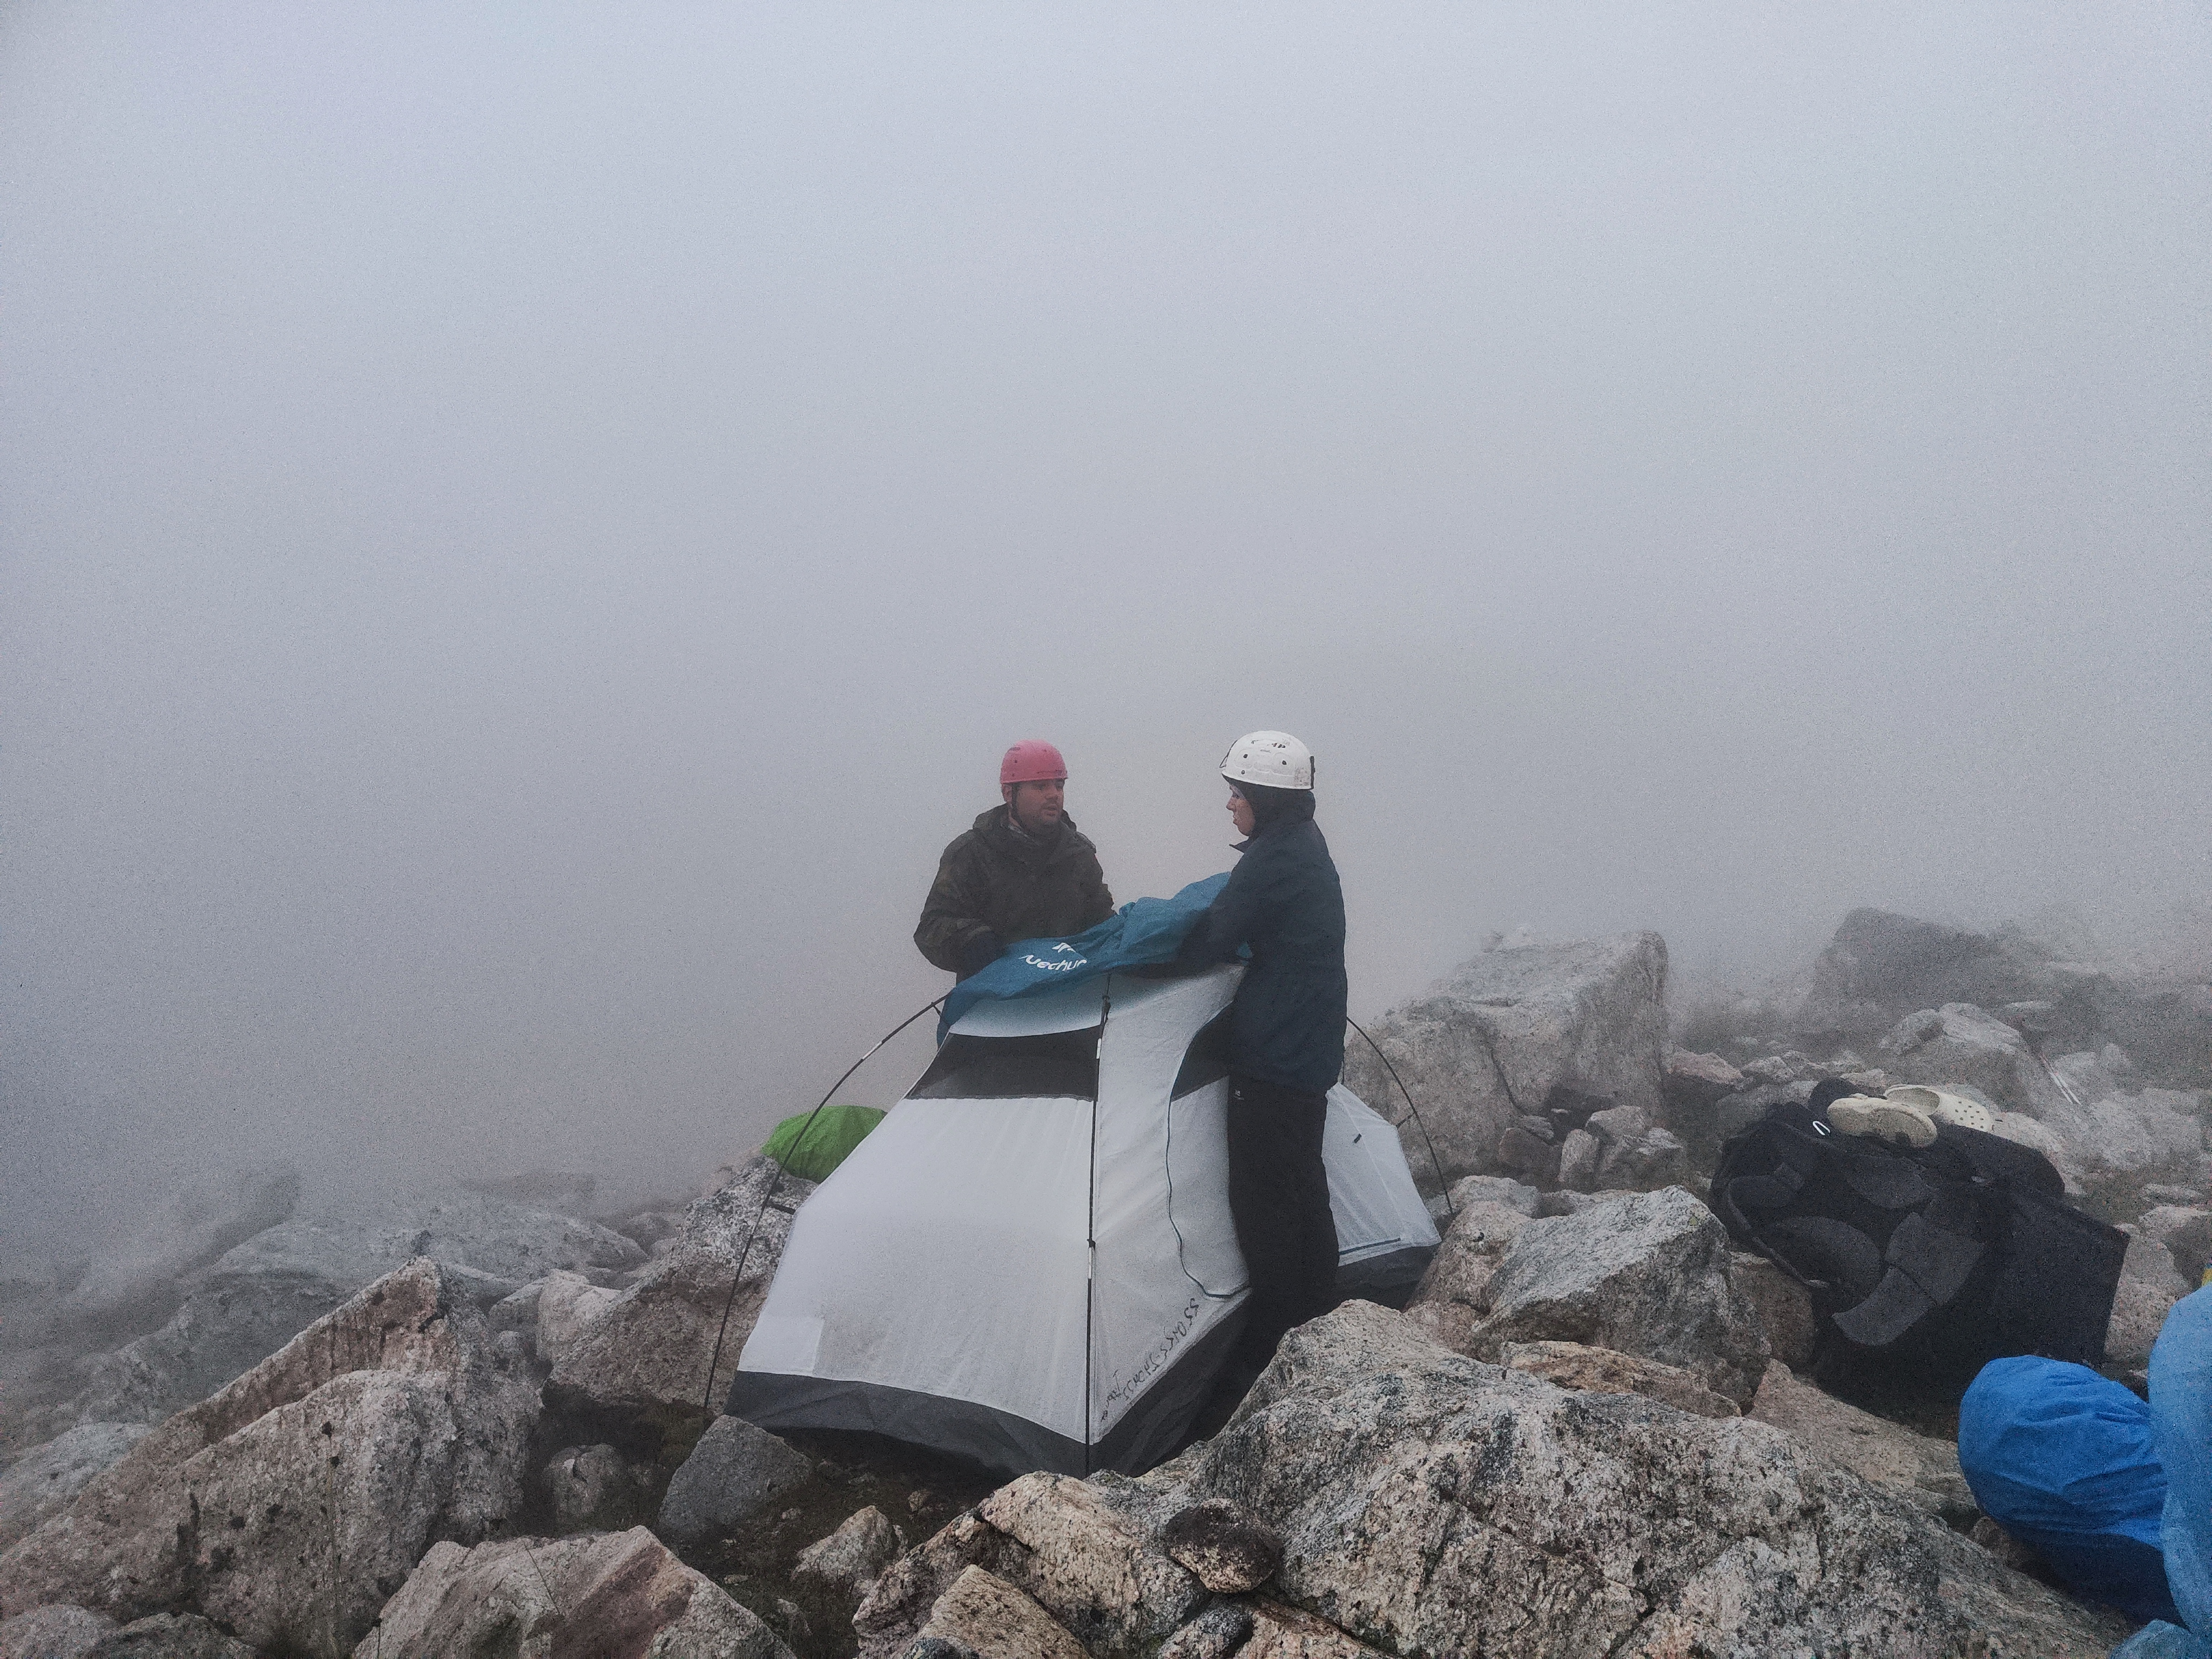
\includegraphics[angle=0, width=0.7\linewidth]{../pics/IMG_20240823_184041}
	\caption{м.н. 23-24 августа}
	\label{fig:IMG_20240823_184041}
\end{figure}

Высота ночёвки в этот день была максимальной за весь поход и составила 3050~м. Неприятным сюрпизом стало то, что источника воды в непосредственной близости от стоянок не оказалось, так как озеро у площадок пересохло. Ближайший источник воды нашёлся в 200~м к западу от м.н., в также почти пересохшем озере, которое спряталось за локальной возвышенностью (<<пупырь>>) около 100~м в диаметре. Относительно этой возвышенности озеро находилось на диаметрально противоположном конце от стоянки. Руководитель сходил на разведку, не дойдя до озера, но услышав воду, --- и по результатам этой разведки стало ясно, что в условиях такого тумана выходить за водой в одиночку крайне опасно. Ситуация была близкой к тому, чтобы не набирать воду вообще, однако в итоге решили выйти половиной группы --- включая руководителя и замруководителя,~--- чтобы в крайнем случае выстроиться в цепочку от озера до лагеря и быть в пределах видимости друг друга. Водоносы взяли с собой навигатор; оставшимся в лагере были выданы инструкции: при любом раскладе оставаться на месте и по истечении контрольного времени подавать голосовые команды. К нашему везению, в момент выхода водоносов из лагеря выдалось погодное окно, во время которого удалось дойти до озера всей группой, не выстраиваясь в цепочку. Пупырь обходили против часовой стрелки по крупной осыпи. 

Пока набирали воду, туман снова стал сгущаться. Путь в обратную сторону по курумнику был не самым приятным, и руководитель по виду рельефа предположил, что с другой стороны есть шансы выйти на травянистый участок, --- а также понадеялся, что тропа, уходящая от м.н. вниз, проходит где-то вблизи пупыря, --- поэтому группа водоносов продолжила обходить пупырь против часовой стрелки. Надежды подсечь тропу оказались ошибочными, а вот рельеф склона действительно сменился на травянистый --- но сам склон стал круче.\alert{(Возможно, я ещё услышала Катины крики именно с этой стороны --- надо уточнить у ребят.)} 

\alert{(Если это не так, то...)} Траверсирование склона в тумане в сумерках, практически полностью <<по приборам>> было достаточно стрессовым занятием. К огромному облегчению, когда до лагеря оставалась треть или четверть круга в обход пупыря, водоносы ясно услышали крики оставшихся в лагере, и, в частности, благодаря им, успешно нащупали дорогу к стоянке. Воду доставили в лагерь, и группа смогла приготовить горячий ужин. Весь выход за водой занял около 40 мин.

\begin{figure}[h!]	
	\centering
	\includegraphics[angle=0, width=0.7\linewidth]{../pics/IMG_20240823_205116}
	\caption{Звёздное небо}
	\label{fig:IMG_20240823_205116}
\end{figure}
 
Примерно в 21:00 туман рассеялся, и нам открылся потрясающий вид на Млечный путь (рис.~\ref{fig:IMG_20240823_205116}).
 
 \begin{table}[h!]
 	\centering
 	\begin{tabular}{|c|c|c|c|c|c|} 
 		\hline 
 		Этап & ЧХВ \\ 	
 		\hline 
 		От т/б <<Глобус>> до начала подъёма в д.р. Джалпаккол  & 00:44 \\
 		Подъём в д.р. Джалпаккол  & 02:33 \\
 		Подъём по д.р. Джалпаккол & 01:17\\ 
 		Подъём в д.р. Кичкинекол Джалпаккольский до подножия моренных валов & 02:08\\ 
 		По моренным валам до перевального взлёта & 03:42\\ 
 		По леднику & 00:28 \\
 		По скалам на седловину & 00:45 \\
 		Спуск к озеру & 00:40 \\
 		Спуск к ночёвкам на 3000 м & 01:51 \\
 		Спуск в д.р. Мырды & 02:08 \\
 		По д.р. Мырды до а/л <<Узункол>>& 01:45 \\
 		\hline
 		\textsc{Полное время подъёма на перевал  }& 10:37\\
 		\textsc{Полное время спуска с перевала }& 06:24 \\
 		\textsc{	Полное время прохождения перевала }& 17:01 \\
 		\hline
 	\end{tabular}
 	\caption{Расклад времени, пер. Джалпаккол Северный}
 \end{table}
 
 \paragraph{Выводы и рекомендации:} пер. Джалпаккол Северный соответствует заявленной категории трудности, разнообразен с точки зрения рельефа, однако может быть утомителен морально при движении по моренным валам. Перевал является хоршей обзорной точкой района, что с лихвой оправдывает утомительность подъёма. Перевал рекомендуется к прохождению в новичковых походах; впрочем, вероятно, не стоит ставить его первым на маршруте, если есть сомнения в физической и моральной подготовке группы.
 
\clearpage
